
In this section, the results of the regression cases (burnup, enrichment, and
time since irradiation) are presented. For each prediction parameter, the plot
format described in Figure \ref{fig:detdemo} is used to show the \gls{MAPE} for
each of the three energy window lists.  However, while seeing the performance
decrease with all three algorithms on the same plot is helpful for getting a
bigger picture of the results, a more detailed visual is also helpful. 

Introduced in Section \ref{sec:sfcoreg}, box plots provide increased
statistical detail and a direct comparison of mean and median error for each
data point, which each taken alone can paint a drastically different picture of
the results. These box plots have a small variation from the original
description, however.  The \gls{MAE} is now represented by black triangles,
since many are above the 75\% quartile level (i.e., outside of the box).  The
\gls{MedAE} remains represented by a white line, which may be hard to see in
some plots because many median errors are near zero.

There is one set of boxes for each algorithm for a given energy window
list-based set of detector training sets.  Because these are box plots, they
are not oriented to the "higher is better" standard of the vertical axis of
the original prediction performance plots.  There are the same red baselines,
but they are now at a positive value since the vertical axis is no longer
negative. In order to see the spread of the data and compare the mean and
median errors, the outliers were suppressed from the box plots. There are many
outliers in these results, and the values can be quite large. Each set of box
plots is therefore repeated with a set of box plots with the outliers included.

Lastly, the full knowledge cases (the 29 nuclide masses, and the 32, 12, and 7
nuclide activities sets) are not able to be represented on the same scale as
the detector training set results, so they are excluded from the box plot
figures. 

\subsubsection{Burnup Regression}

\begin{figure}[!htb]
  \centering
  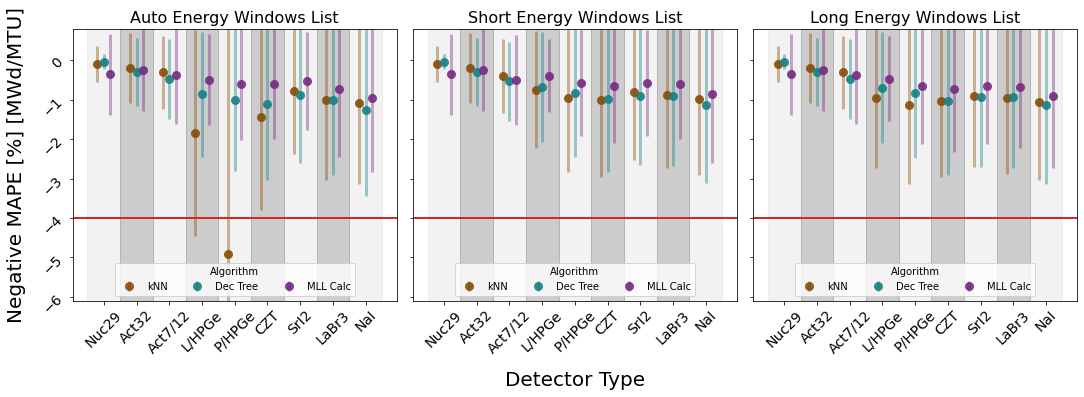
\includegraphics[width=\textwidth]{./chapters/exp2/detector_preds_wrt_enlist_MAPE_burn.png}
  \caption[Prediction performance of burnup regression with decreasing detector 
           energy resolution]
          {Prediction performance of burnup measured by \acrshort{MAPE} with 
           respect to decreasing detector energy resolution for three types 
           of processed gamma spectra.}
  \label{fig:burn}
\end{figure}

\begin{figure}[!hp]
  \centering
  \begin{subfigure}[b]{\textwidth}
    \centering
    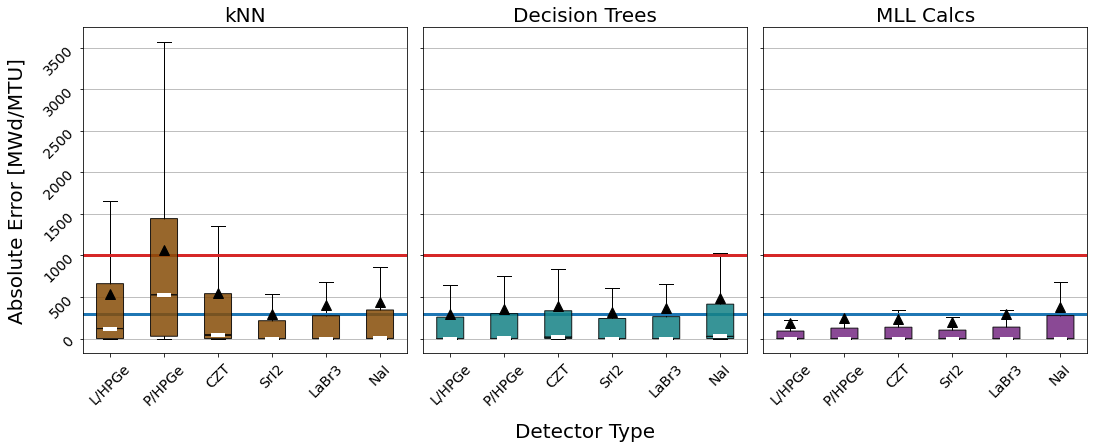
\includegraphics[width=0.92\textwidth]{./chapters/exp2/abserror_boxplots_auto_burn.png}
    \caption{Burnup prediction error box plots for auto energy windows list.}
    \label{fig:burnboxA}
  \end{subfigure}
  \vskip\baselineskip
  \begin{subfigure}[b]{\textwidth}
    \centering
    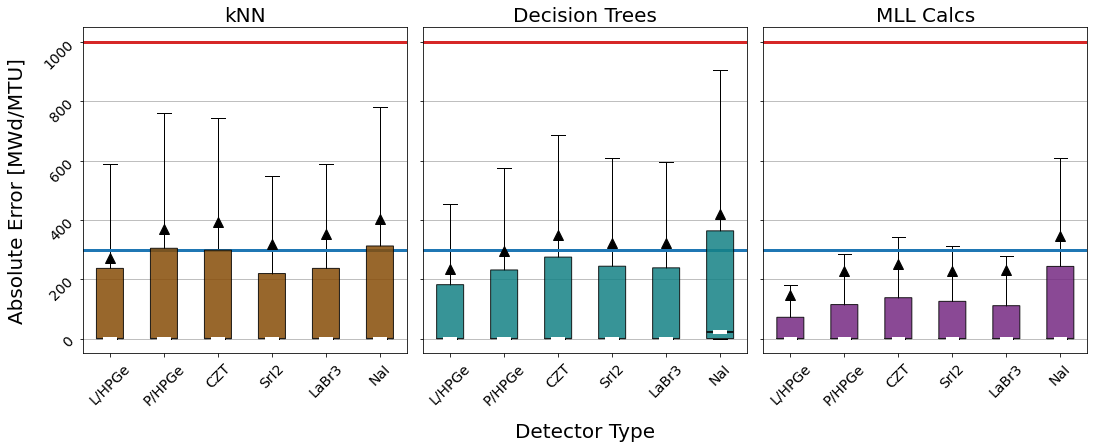
\includegraphics[width=0.92\textwidth]{./chapters/exp2/abserror_boxplots_short_burn.png}
    \caption{Burnup prediction error box plots for short energy windows list.}
    \label{fig:burnboxB}
  \end{subfigure}
  \vskip\baselineskip
  \begin{subfigure}[b]{\textwidth}
    \centering
    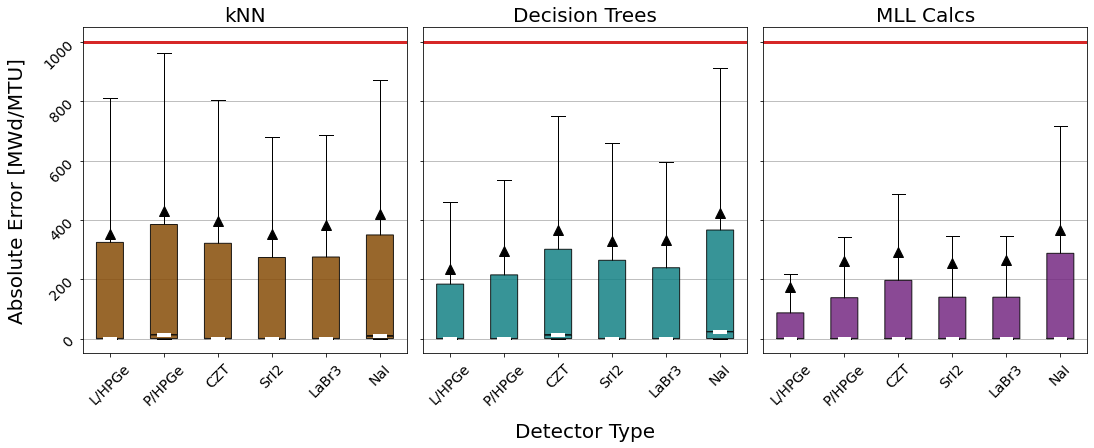
\includegraphics[width=0.92\textwidth]{./chapters/exp2/abserror_boxplots_long_burn.png}
    \caption{Burnup prediction error box plots for long energy windows list.}
    \label{fig:burnboxC}
  \end{subfigure}
  \caption[Box plots (without outliers) of burnup regression for six detectors]
          {Prediction performance of burnup for six detectors as shown by box 
           plots \emph{without} outliers shown.}
  \label{fig:burnbox}
\end{figure}

\begin{figure}[!hp]
  \centering
  \begin{subfigure}[b]{\textwidth}
    \centering
    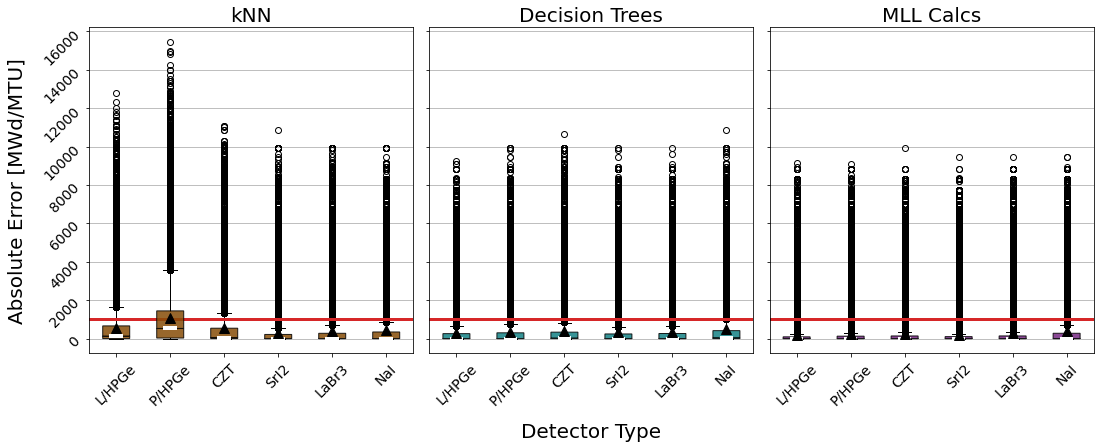
\includegraphics[width=0.92\textwidth]{./chapters/exp2/abserror_boxplots_outliers_auto_burn.png}
    \caption{Burnup prediction error box plots for auto energy windows list.}
    \label{fig:burnboxflyA}
  \end{subfigure}
  \vskip\baselineskip
  \begin{subfigure}[b]{\textwidth}
    \centering
    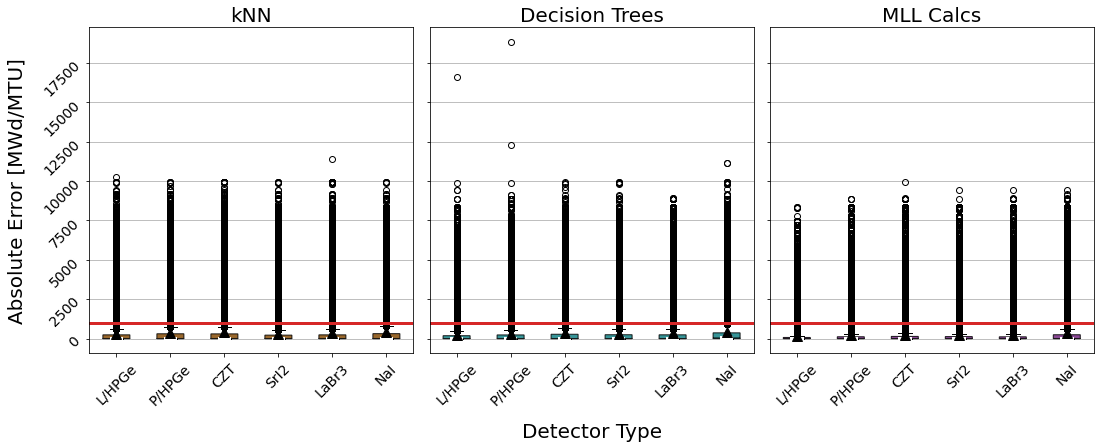
\includegraphics[width=0.92\textwidth]{./chapters/exp2/abserror_boxplots_outliers_short_burn.png}
    \caption{Burnup prediction error box plots for short energy windows list.}
    \label{fig:burnboxflyB}
  \end{subfigure}
  \vskip\baselineskip
  \begin{subfigure}[b]{\textwidth}
    \centering
    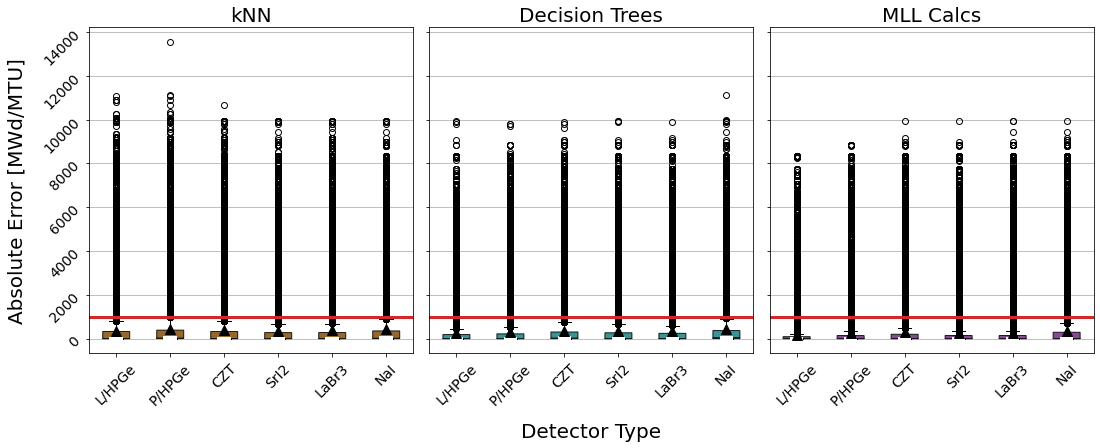
\includegraphics[width=0.92\textwidth]{./chapters/exp2/abserror_boxplots_outliers_long_burn.png}
    \caption{Burnup prediction error box plots for long energy windows list.}
    \label{fig:burnboxflyC}
  \end{subfigure}
  \caption[Box plots (with outliers) of burnup regression for six detectors]
          {Prediction performance of burnup for six detectors as shown by box 
           plots \emph{with} outliers shown.}
  \label{fig:burnboxfly}
\end{figure}

The baseline performance in Figure \ref{fig:burn} is at -4\% \gls{MAPE} for
burnup, chosen by the lowest performance of the three algorithms at the
reference point of 20\% training set error for the 29 nuclide mass training set
in Figure \ref{fig:burnmape}. In Figures \ref{fig:burnbox} and
\ref{fig:burnboxfly}, the red baseline is at $1000\:MWd/MTU$, from the
reference point in Figure \ref{fig:burnmae}.  In these two sets of plots, the
baseline is at a positive value because the box plots do not have a negative
vertical axis. 

Figure \ref{fig:burn} shows encouraging results about the burnup prediction
for all three algorithms and all three energy windows lists used to process the
gamma spectra. There is overall a gradual decrease from perfect knowledge
starting at close to 0\% error to the lowest energy resolution detector at
about -1.5\%.  There are two anomalous cases, as with the reactor type results
in Figure \ref{fig:rxtr}: the predictions using \textit{k}-nearest neighbors
for the two \gls{HPGe} detectors processed with the auto energy windows list.
The reason for this behavior is discussed at the end of Section
\ref{sec:exp2_rxtr}. 

Next, in Figures \ref{fig:burnbox} and \ref{fig:burnboxfly} the vertical axis
orientation flips to positive absolute error, so that higher values are worse
and the goal is to have the mean and median errors be below the red line.  Most
of the burnup errors in Figures \ref{fig:burnboxA}, \ref{fig:burnboxB}, and
\ref{fig:burnboxC} are below the red line, except for the \gls{MAE} from the
portable \gls{HPGe}. This set of errors from the portable\gls{HPGe} also
encompass a range than reaches up to $>3500\:MWd/MTU$, which is about $4x$
higher than the other box plots in all three subfigures. 

The burnup predictions for the most part perform better than the red line, for
all algorithms and gamma spectra-processing methods.  Of course, the \gls{MLL}
calculations consistently have the lowest errors. In all but the two \gls{HPGe}
cases with the auto energy windows list, the \gls{MedAE}s are close to zero.
This indicates that there are very good predictions for at least half of the
training set.  However, the \gls{MAE}s are all above the 75\% quartile, which
suggests the errors that do exist are quite large relative to the interquartile
range.  

Furthermore, looking at the sets of box plots with outliers present in Figure
\ref{fig:burnboxfly} shows that there are many errors far outside of the full
range of burnup errors that reach up to almost $20000\:MWd/MTU$ (for decision
trees with the short energy windows list in Figure \ref{fig:burnboxflyB}), an
error that has a magnitude of about 30\% of the largest burnup value in the
training set.  Figure \ref{fig:burn} shows that these large \gls{MAE}s are
actually are of low relative error with the data points all being above -1.5\%.
The number of outliers ranges from an average between $53k$ and $65k$ per box
for the two scikit-learn algorithms, and about $76k$ per box for the \gls{MLL}
calculations.  This means that $12-17\%$ of the training set samples are
outliers.  The high magnitude errors along with the large number of outliers
contributes to the standard deviations in Figure \ref{fig:burn}, which are so
large that it is difficult to conclusively define a trend.

\subsubsection{\texorpdfstring{${}^{235}\text{U}$}{U-235} Enrichment Regression}

\begin{figure}[!htb]
  \centering
  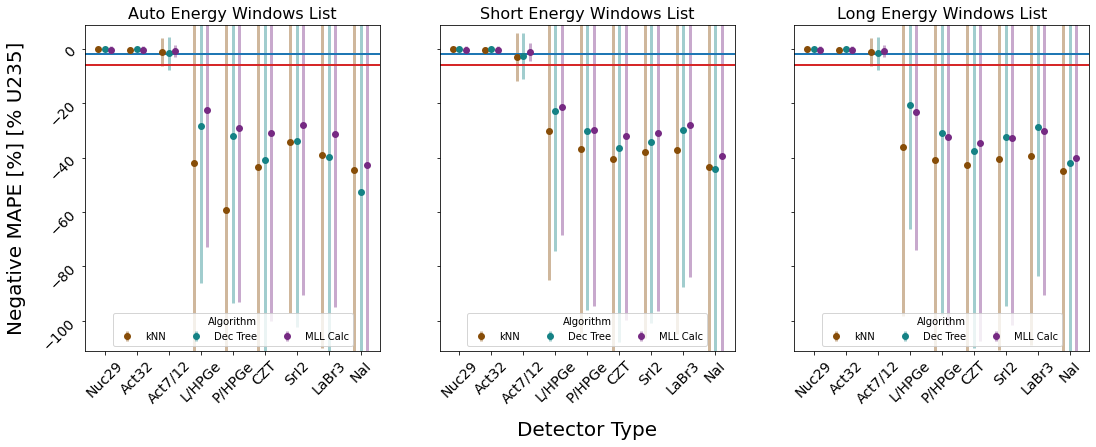
\includegraphics[width=\textwidth]{./chapters/exp2/detector_preds_wrt_enlist_MAPE_enri.png}
  \caption[Prediction performance of \acrshort{U235} regression with decreasing 
           detector energy resolution]
          {Prediction performance of \acrshort{U235} enrichment measured by 
           \acrshort{MAPE} with respect to decreasing detector energy resolution
           for three types of processed gamma spectra.}
  \label{fig:enri}
\end{figure}

\begin{figure}[!hp]
  \centering
  \begin{subfigure}[b]{\textwidth}
    \centering
    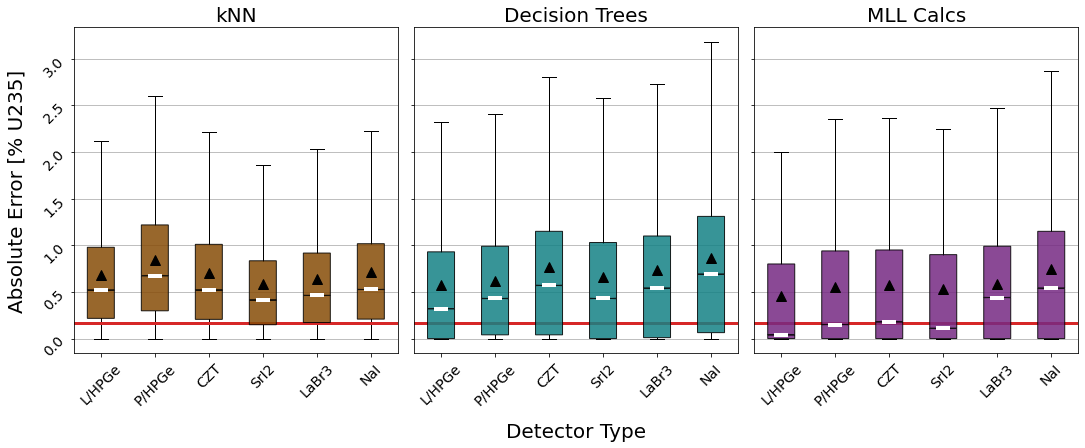
\includegraphics[width=0.92\textwidth]{./chapters/exp2/abserror_boxplots_auto_enri.png}
    \caption{\gls{U235} enrichment prediction error box plots for auto energy windows list.}
    \label{fig:enriboxA}
  \end{subfigure}
  \vskip\baselineskip
  \begin{subfigure}[b]{\textwidth}
    \centering
    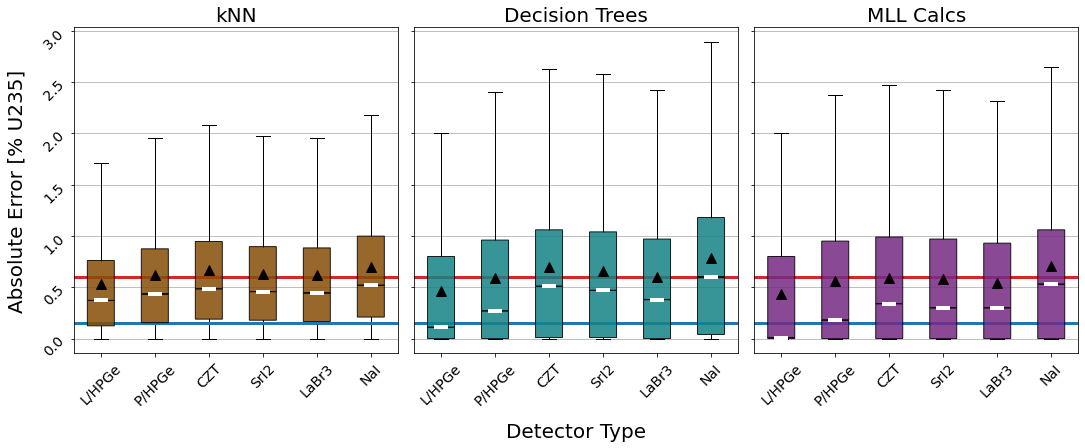
\includegraphics[width=0.92\textwidth]{./chapters/exp2/abserror_boxplots_short_enri.png}
    \caption{\gls{U235} enrichment prediction error box plots for short energy windows list.}
    \label{fig:enriboxB}
  \end{subfigure}
  \vskip\baselineskip
  \begin{subfigure}[b]{\textwidth}
    \centering
    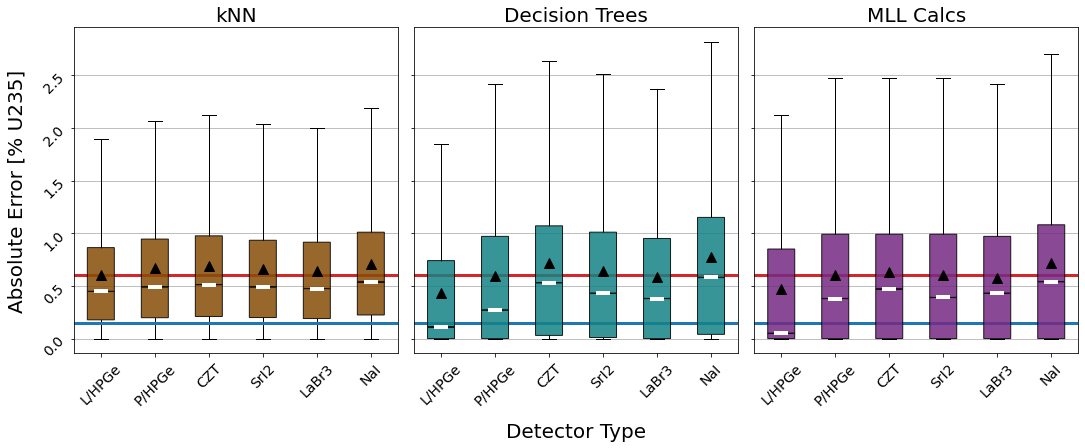
\includegraphics[width=0.92\textwidth]{./chapters/exp2/abserror_boxplots_long_enri.png}
    \caption{\gls{U235} enrichment prediction error box plots for long energy windows list.}
    \label{fig:enriboxC}
  \end{subfigure}
  \caption[Box plots (without outliers) of \acrshort{U235} enrichment regression 
           for six detectors]
          {Prediction performance of \acrshort{U235} enrichment for six detectors 
           as shown by box plots \emph{without} outliers shown.}
  \label{fig:enribox}
\end{figure}

\begin{figure}[!hp]
  \centering
  \begin{subfigure}[b]{\textwidth}
    \centering
    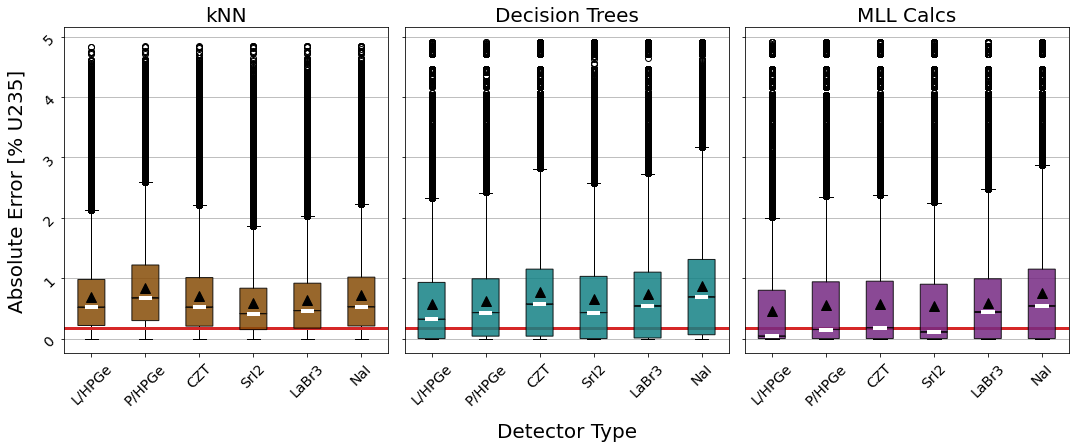
\includegraphics[width=0.914\textwidth]{./chapters/exp2/abserror_boxplots_outliers_auto_enri.png}
    \caption{\gls{U235} enrichment prediction error box plots for auto energy windows list.}
    \label{fig:enriboxflyA}
  \end{subfigure}
  \vskip\baselineskip
  \begin{subfigure}[b]{\textwidth}
    \centering
    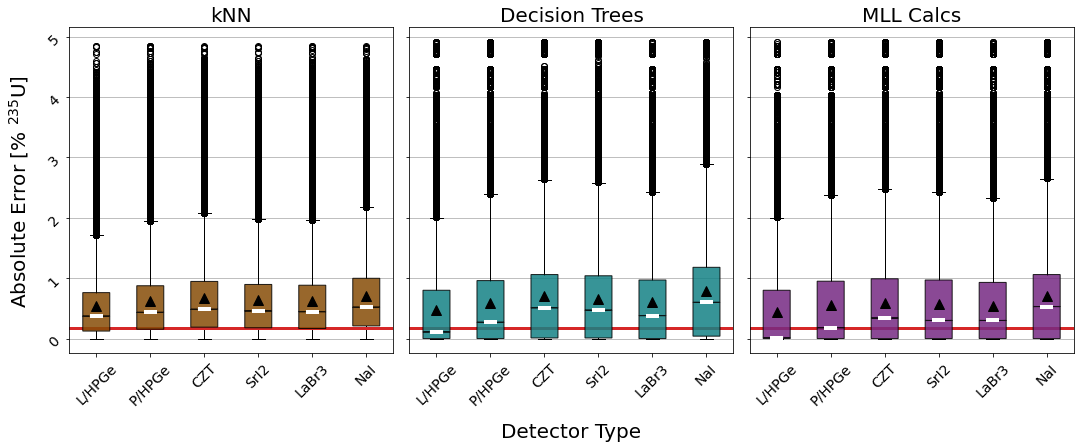
\includegraphics[width=0.914\textwidth]{./chapters/exp2/abserror_boxplots_outliers_short_enri.png}
    \caption{\gls{U235} enrichment prediction error box plots for short energy windows list.}
    \label{fig:enriboxflyB}
  \end{subfigure}
  \vskip\baselineskip
  \begin{subfigure}[b]{\textwidth}
    \centering
    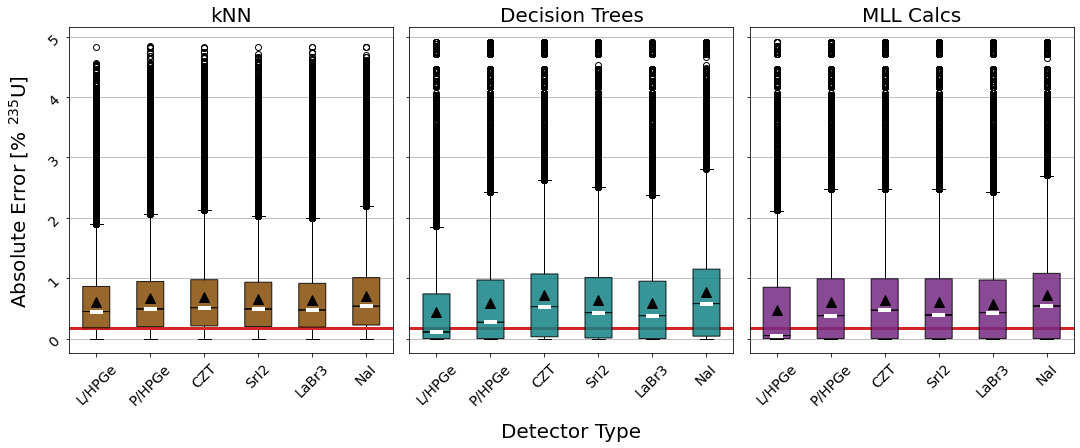
\includegraphics[width=0.914\textwidth]{./chapters/exp2/abserror_boxplots_outliers_long_enri.png}
    \caption{\gls{U235} enrichment prediction error box plots for long energy windows list.}
    \label{fig:enriboxflyC}
  \end{subfigure}
  \caption[Box plots (with outliers) of \acrshort{U235} enrichment regression
           for six detectors] 
          {Prediction performance of \acrshort{U235} enrichment for six 
           detectors as shown by box plots \emph{with} outliers shown.}
  \label{fig:enriboxfly}
\end{figure}

The baseline performance for the enrichment predictions in Figure
\ref{fig:enri} is at -6\% \gls{MAPE}, chosen by the lowest performance of the
three algorithms at the reference point of 20\% training set error for the 29
nuclide mass training set in in Figure \ref{fig:enrimape}. In Figures
\ref{fig:enribox} and \ref{fig:enriboxfly}, the red baseline is at
$0.17\:\%\:{}^{235}\text{U}$, from the reference point in Figure
\ref{fig:enrimae}.  In these two sets of plots, the baseline is at a positive
value because the box plots do not have a negative vertical axis. 

Figure \ref{fig:enri} shows discouraging results about the \gls{U235}
enrichment prediction for all three algorithms and all three energy windows
lists used to process the gamma spectra.  Taken as a whole, the data points in
Figure \ref{fig:enri} have a distinct shape, similar to the behavior in Figure
\ref{fig:rxtr}.  The three full knowledge cases have near-perfect enrichment
prediction and the six detectors for all three energy windows lists are nearly
flat, where most data points are in the -50\% to -30\% range. This is a large
range but also a high relative error.  As with the other previously discussed
prediction types, there are two anomalous cases: the prediction using
\textit{k}-nearest neighbors for the two \gls{HPGe} detectors processed with
the auto energy windows list. The reason for this behavior is discussed at the
end of Section \ref{sec:exp2_rxtr}. In this set of results, \textit{k}-nearest
neighbors usually performs the worst or, when it does not, about equal to
decision trees. The \gls{MLL} calculations are the best performing for the auto
energy windows list, but the results in the short and long energy windows lists
shows decision trees performing close to and sometimes outperforming \gls{MLL}.

Next, in Figures \ref{fig:enribox} and \ref{fig:enriboxfly} the vertical axis
orientation flips to positive absolute error, so that higher values are worse
and the goal is to have the mean and median errors be below the red line.
Unlike with the burnup errors being mostly below the red line in Figure
\ref{fig:burnbox}, this is not the case for enrichment. None of the \gls{MAE}s
are below the red line, and the majority of the \gls{MedAE}s are also above it.
There are a few box plots where the \gls{MedAE} is below the red line: the
first four detectors processed with the auto energy windows list as predicted
using \gls{MLL}, and the lab-based \gls{HPGe} processed with both the short and
long lists for decision trees and \gls{MLL} calculations.  Interestingly, the
red line appears to run across the bottom quartile for the \textit{k}-nearest
neighbor predictions for all three energy windows lists, which indicates about
25\% of those predictions are below the level considered acceptable here.  

The range of errors reaches to about $3\:\%\:{}^{235}\text{U}$ without
outliers, which is a large magnitude since the maximum enrichment is about
$5\:\%\:{}^{235}\text{U}$. All nine combinations of algorithm and energy
windows list in Figure \ref{fig:enriboxfly} have outliers that reach the full
$5\:\%\:{}^{235}\text{U}$, indicating that some of the 0.5\% enriched fuels are
being mispredicted at a 5\% level.  Furthermore, an error that large is of the
magnitude of the highest enrichment level in the training set.  The number of
outliers ranges from an average of about $18k$ for the \textit{k}-nearest
neighbors boxes, and about $14k$ per box for the decision trees and \gls{MLL}
calculations, meaning about 3-4\% of the training set samples are outliers.
Although there are much fewer outliers than with the burnup predictions, the
wide range of \gls{MAE} magnitudes and the large \gls{MAPE}s contribute to the
large standard deviations in Figure \ref{fig:enri}. Again, the standard
deviations are so large that it is difficult to conclusively define a trend.

\subsubsection{Time Since Irradiation Regression}

\begin{figure}[!htb]
  \centering
  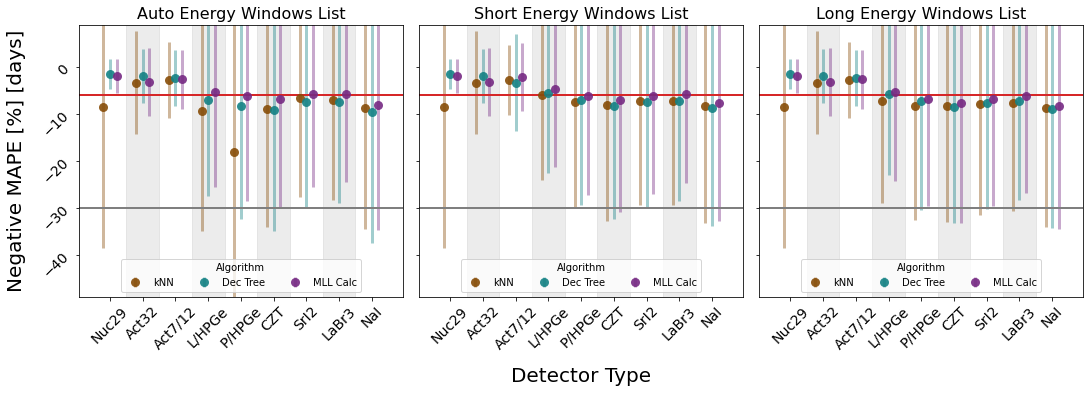
\includegraphics[width=\textwidth]{./chapters/exp2/detector_preds_wrt_enlist_MAPE_cool.png}
  \caption[Prediction performance of time since irradiation regression with 
           decreasing detector energy resolution]
           {Prediction performance of time since irradiation measured by 
           \acrshort{MAPE} with respect to decreasing detector energy resolution
           for three types of processed gamma spectra.}
  \label{fig:cool}
\end{figure}

\begin{figure}[!hp]
  \centering
  \begin{subfigure}[b]{\textwidth}
    \centering
    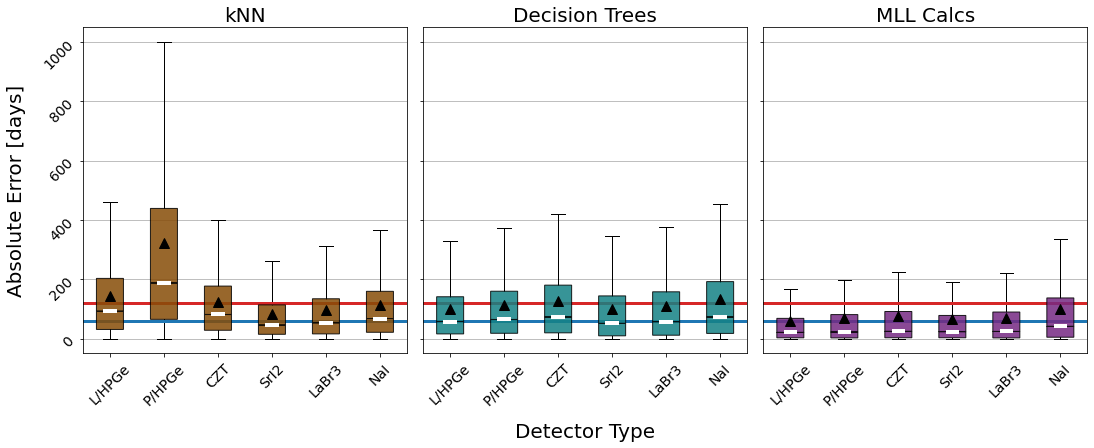
\includegraphics[width=0.92\textwidth]{./chapters/exp2/abserror_boxplots_auto_cool.png}
    \caption{Time since irradiation prediction performance box plots for auto energy windows list.}
    \label{fig:coolboxA}
  \end{subfigure}
  \vskip\baselineskip
  \begin{subfigure}[b]{\textwidth}
    \centering
    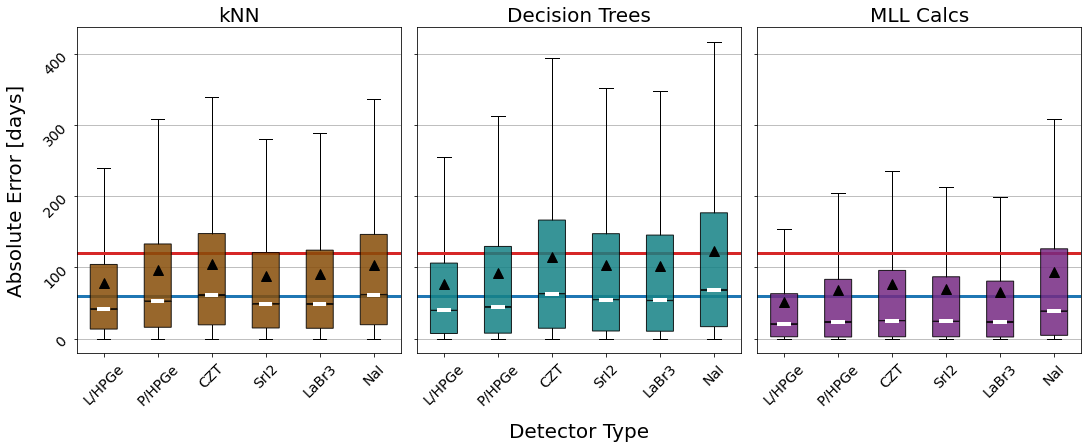
\includegraphics[width=0.92\textwidth]{./chapters/exp2/abserror_boxplots_short_cool.png}
    \caption{Time since irradiation prediction performance box plots for short energy windows list.}
    \label{fig:coolboxB}
  \end{subfigure}
  \vskip\baselineskip
  \begin{subfigure}[b]{\textwidth}
    \centering
    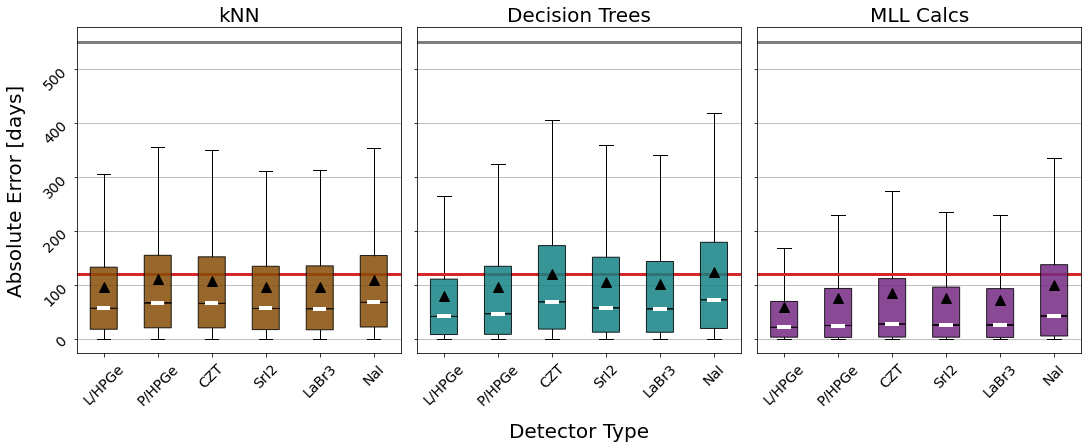
\includegraphics[width=0.92\textwidth]{./chapters/exp2/abserror_boxplots_long_cool.png}
    \caption{Time since irradiation prediction performance box plots for long energy windows list.}
    \label{fig:coolboxC}
  \end{subfigure}
  \caption[Box plots (without outliers) of time since irradiation regression 
           for six detectors]
          {Prediction performance of time since irradiation for six detectors as 
           shown by box plots \emph{without} outliers shown.}
  \label{fig:coolbox}
\end{figure}

\begin{figure}[!hp]
  \centering
  \begin{subfigure}[b]{\textwidth}
    \centering
    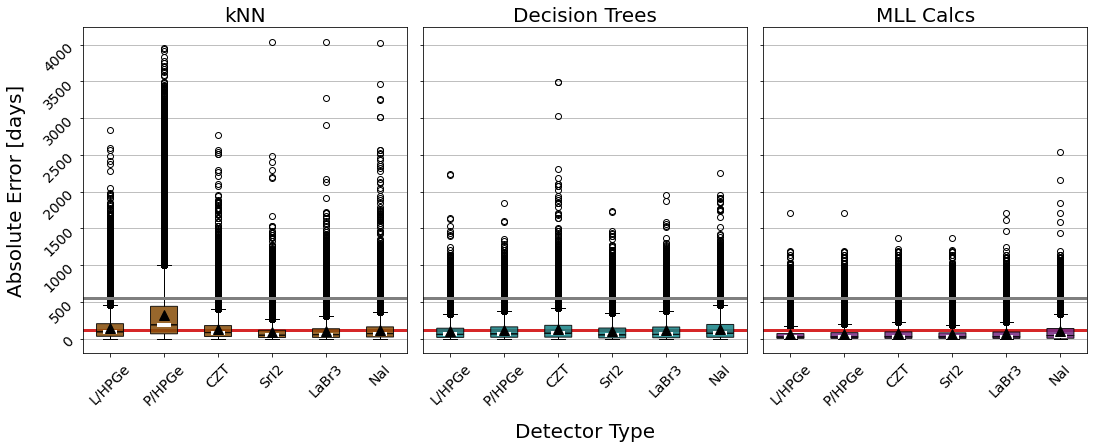
\includegraphics[width=0.92\textwidth]{./chapters/exp2/abserror_boxplots_outliers_auto_cool.png}
    \caption{Time since irradiation prediction performance box plots for auto energy windows list.}
    \label{fig:coolboxflyA}
  \end{subfigure}
  \vskip\baselineskip
  \begin{subfigure}[b]{\textwidth}
    \centering
    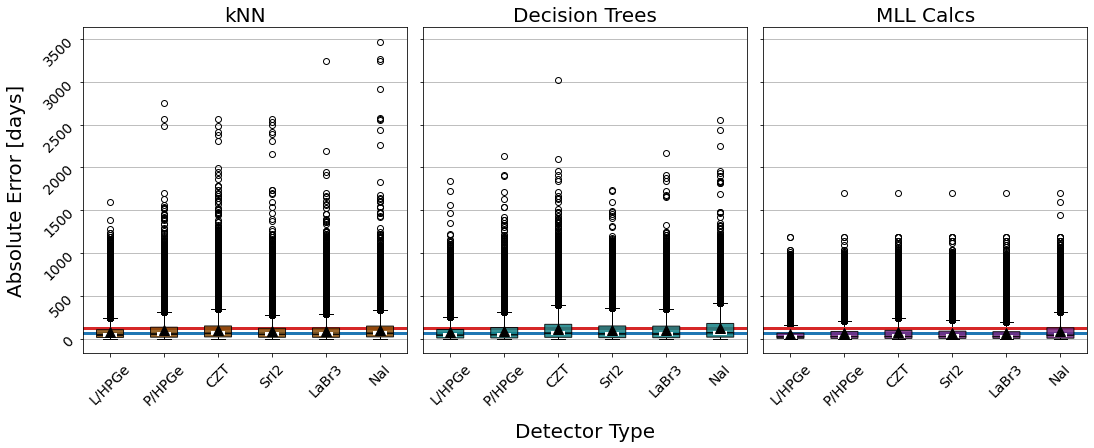
\includegraphics[width=0.92\textwidth]{./chapters/exp2/abserror_boxplots_outliers_short_cool.png}
    \caption{Time since irradiation prediction performance box plots for short energy windows list.}
    \label{fig:coolboxflyB}
  \end{subfigure}
  \vskip\baselineskip
  \begin{subfigure}[b]{\textwidth}
    \centering
    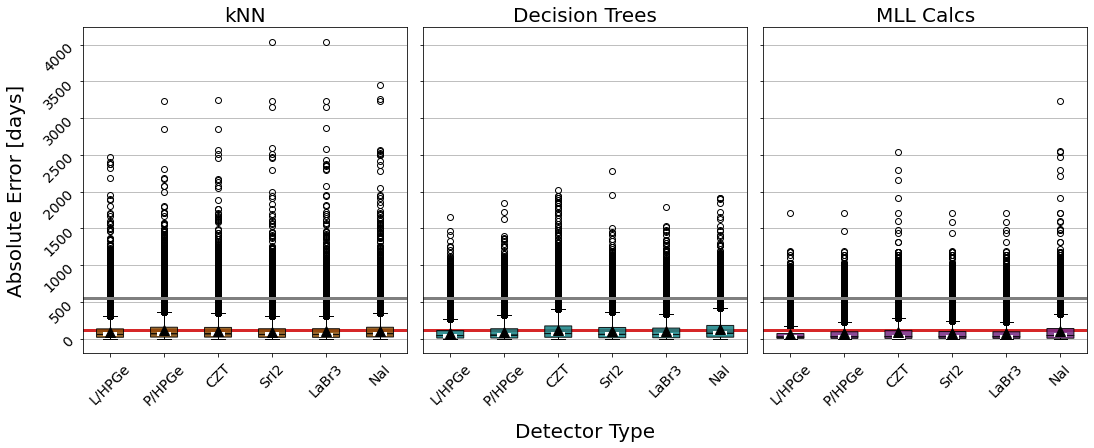
\includegraphics[width=0.92\textwidth]{./chapters/exp2/abserror_boxplots_outliers_long_cool.png}
    \caption{Time since irradiation prediction performance box plots for long energy windows list.}
    \label{fig:coolboxflyC}
  \end{subfigure}
  \caption[Box plots (with outliers) of time since irradiation regression for 
           six detectors]
          {Prediction performance of time since irradiation for six detectors as 
           shown by box plots \emph{with} outliers shown.}
  \label{fig:coolboxfly}
\end{figure}

The original baseline performance for the time since irradiation predictions in
Figure \ref{fig:cool} were at -30\% \gls{MAPE}, chosen by the lowest
performance of the three algorithms at the reference point of 20\% training set
error for the 29 nuclide mass training set in in Figure \ref{fig:coolmape}.
However, the \textit{k}-nearest neighbors algorithm in that plot had
exceptionally poor performance compared to the other two algorithms, so all of
the results from the detector-based training sets (including those predicted
using \textit{k}-nearest neighbors, oddly enough) far outperform this baseline.
Therefore, a new one was chosen based on the decision trees performance at the
reference point in Figure \ref{fig:coolmape}, at a \gls{MAPE} of -6\%.
Similarly, in Figures \ref{fig:coolbox} and \ref{fig:coolboxfly}, the original
baseline is at $550\:days$ and the updated red baseline is at $120\:days$, from
the \textit{k}-nearest neighbors and decision trees performances, respectively,
at the reference point in Figure \ref{fig:coolmae}.  In these two sets of
plots, the baseline is at a positive value because the box plots do not have a
negative vertical axis. 

Figure \ref{fig:cool} shows the relative error results from the time since
irradiation prediction for all three algorithms and all three energy windows
lists used to process the gamma spectra. There is a gradual decrease from
perfect knowledge, in contrast to enrichment but similar to burnup, starting at
close to -2\% error to the lowest energy resolution detector at about -10\%.
The red line in these plots makes for an interesting delineation of the
results, since there are 2 or 3 \gls{MLL} data points in each plot that are on
or exceed the baseline.  Additionally, the decision trees data points for the
lab-based \gls{HPGe} for the short and long energy windows lists also exceed
the baseline. The remainder of the detector-based training sets are below the
baseline.  Notably, the \textit{k}-nearest neighbors case with the 29 nuclide
masses training set is below the line at about -10\%.  This is from the
previously mentioned issues with this algorithm's performance with this
particular prediction parameter.  For reactor type, burnup, and enrichment, the
predictions using \textit{k}-nearest neighbors for the two \gls{HPGe} detectors
processed with the auto energy windows list performed drastically worse than
the rest of the scenarios. For time since irradiation, however, this is only
true for the portable \gls{HPGe}.  The reason for this behavior is discussed at
the end of Section \ref{sec:exp2_rxtr}. 

Next, in Figures \ref{fig:coolbox} and \ref{fig:coolboxfly} the vertical axis
orientation flips to positive absolute error, so that higher values are worse
and the goal is to have the mean and median errors be below the red line.  The
auto energy windows list results in Figure \ref{fig:coolboxA} have many of the
\gls{MAE}s and all of the \gls{MedAE}s below the red line.  The \gls{MAE}s of
the two \gls{HPGe}s for \textit{k}-nearest neighbors are above it, and the
\gls{CZT} and \gls{NaI} detectors for decision trees are above it as well.
Nearly all of the cooling time errors in Figures \ref{fig:coolboxB}, and
\ref{fig:coolboxC} are on or below the red line, except for the \gls{MAE} of
the decision trees results for the \gls{NaI} detector.  Other than the portable
\gls{HPGe} box which encompasses a range reaching $1000\:days$, the range of
absolute errors rarely exceeds $400\:days$, or a little over a year.  Taking an
aggregate view of the three plots, many of the \gls{MAE}s are around
$100\:days$.

Although the range of absolute errors typically reaches to around $400\:days$,
the outliers in Figure \ref{fig:coolboxfly} reach to about $10x$ that level to
approximately $4000\:days$. This error magnitude is about 70\% of the largest
time since irradiation level in the training set.  The number of outliers have
an average of about $26k$ per box for the two scikit-learn algorithms, and
about $41k$ per box for the \gls{MLL} calculations.  This means that $6-9\%$ of
the training set samples are outliers.  The high magnitude errors along with
the large number of outliers contributes to the standard deviations in Figure
\ref{fig:cool}, which are so large that it is difficult to conclusively define
a trend.
